\documentclass[11pt]{article}

%%%%%%%%%%%%%%%%%%%%%%%%%%%%%%%%%%%%%%%%
% PACKAGES
%%%%%%%%%%%%%%%%%%%%%%%%%%%%%%%%%%%%%%%%
\usepackage[margin=1in]{geometry}
\usepackage{amsmath,amsfonts,amssymb}
\usepackage{xcolor}
\usepackage{graphicx}
\usepackage{tikz}
\usetikzlibrary{arrows.meta, positioning, shapes.geometric, calc}
\usepackage{hyperref}
\usepackage{enumitem}
\usepackage{titlesec}
\usepackage{array}
\usepackage{listings}

%%%%%%%%%%%%%%%%%%%%%%%%%%%%%%%%%%%%%%%%
% COLOR SCHEME (black/blue/red)
%%%%%%%%%%%%%%%%%%%%%%%%%%%%%%%%%%%%%%%%
\definecolor{myblue}{RGB}{20,90,160}
\definecolor{myred}{RGB}{180,40,40}
\definecolor{mygreen}{RGB}{20,120,70}
\newcommand{\blue}[1]{\textcolor{myblue}{#1}}
\newcommand{\red}[1]{\textcolor{myred}{#1}}
\newcommand{\green}[1]{\textcolor{mygreen}{#1}}

\hypersetup{
  colorlinks=true,
  linkcolor=myblue,
  urlcolor=myblue,
  citecolor=myblue
}

%%%%%%%%%%%%%%%%%%%%%%%%%%%%%%%%%%%%%%%%
% SECTION STYLING
%%%%%%%%%%%%%%%%%%%%%%%%%%%%%%%%%%%%%%%%
\titleformat{\section}
{\large\bfseries\color{myblue}}
{\thesection}{1em}{}

\titleformat{\subsection}
{\bfseries\color{myblue}}
{\thesubsection}{1em}{}

%%%%%%%%%%%%%%%%%%%%%%%%%%%%%%%%%%%%%%%%
% MEMORY BOXES (same structure as your doc)
%%%%%%%%%%%%%%%%%%%%%%%%%%%%%%%%%%%%%%%%
\newenvironment{bluebox}
{\vspace{6pt}\noindent\begin{tikzpicture}
\node[
draw=myblue, line width=1pt,
rounded corners=6pt,
inner sep=8pt,
text width=\dimexpr\linewidth-20pt\relax
]\bgroup
\begin{minipage}{\dimexpr\linewidth-32pt\relax}
\blue{\textbf{Key Idea}}\par\vspace{4pt}}
{\end{minipage}\egroup;\end{tikzpicture}\vspace{6pt}}

\newenvironment{redbox}
{\vspace{6pt}\noindent\begin{tikzpicture}
\node[
draw=myred, line width=1pt,
rounded corners=6pt,
inner sep=8pt,
text width=\dimexpr\linewidth-20pt\relax
]\bgroup
\begin{minipage}{\dimexpr\linewidth-32pt\relax}
\red{\textbf{Important}}\par\vspace{4pt}}
{\end{minipage}\egroup;\end{tikzpicture}\vspace{6pt}}

\newenvironment{importantbox}
{\vspace{6pt}\noindent\begin{tikzpicture}
\node[
draw=myred, line width=1pt,
rounded corners=6pt,
inner sep=8pt,
text width=\dimexpr\linewidth-20pt\relax
]\bgroup
\begin{minipage}{\dimexpr\linewidth-32pt\relax}
\red{\textbf{Important}}\par\vspace{4pt}}
{\end{minipage}\egroup;\end{tikzpicture}\vspace{6pt}}

\newenvironment{addedbox}
{\vspace{6pt}\noindent\begin{tikzpicture}
\node[
draw=mygreen, line width=1pt,
rounded corners=6pt,
inner sep=8pt,
text width=\dimexpr\linewidth-20pt\relax
]\bgroup
\begin{minipage}{\dimexpr\linewidth-32pt\relax}
\green{\textbf{Added Clarification}}\par\vspace{4pt}}
{\end{minipage}\egroup;\end{tikzpicture}\vspace{6pt}}

%%%%%%%%%%%%%%%%%%%%%%%%%%%%%%%%%%%%%%%%
% NOTE SPACE (vague outline, lots of room)
%%%%%%%%%%%%%%%%%%%%%%%%%%%%%%%%%%%%%%%%
\newcommand{\notespace}{\vspace{0.6cm}\hrule\vspace{0.6cm}}
\newcommand{\bigspace}{\vspace{1.0cm}\hrule\vspace{1.0cm}}

%%%%%%%%%%%%%%%%%%%%%%%%%%%%%%%%%%%%%%%%
% CODE STYLE (simple + readable)
%%%%%%%%%%%%%%%%%%%%%%%%%%%%%%%%%%%%%%%%
\lstdefinestyle{mystyle}{
  basicstyle=\ttfamily\small,
  keywordstyle=\color{myblue}\bfseries,
  commentstyle=\color{myred},
  stringstyle=\color{myblue},
  numbers=left,
  numberstyle=\tiny,
  stepnumber=1,
  numbersep=8pt,
  breaklines=true,
  frame=single,
  framerule=0.5pt,
  rulecolor=\color{black},
  showstringspaces=false
}
\lstset{style=mystyle}

%%%%%%%%%%%%%%%%%%%%%%%%%%%%%%%%%%%%%%%%
% DOC HEADER
%%%%%%%%%%%%%%%%%%%%%%%%%%%%%%%%%%%%%%%%
\title{\blue{ML Performance Reading Group Notes} \\ \large }
\author{\textit{EleutherAI}}
\date{}

\begin{document}
\maketitle

%%%%%%%%%%%%%%%%%%%%%%%%%%%%%%%%%%%%%%%%%%%%%%%%%%%%%%%%%%%%
\section{ \textbf{Session 1: GPU Architecture, CUDA, NCCL}}

%%%%%%%%%%%%%%%%%%%%%%%%%%%%%%%%%%%%%%%%%%%%%%%%%%%%%%%%%%%%

%%%%%%%%%%%%%%%%%%%%%%%%%%%%%%%%%%%%%%%%%%%%%%%%%%%%%%%%%%%%
\subsection{High-Level Summary}
%%%%%%%%%%%%%%%%%%%%%%%%%%%%%%%%%%%%%%%%%%%%%%%%%%%%%%%%%%%%
\begin{itemize}[leftmargin=1.3em]

% ============================================================
\item \textbf{GPU Architecture}

\begin{bluebox}
\textbf{One-sentence difference:} CPUs are more \blue{latency-optimized} and GPUs are more \blue{throughput-optimized}.
\end{bluebox}

So what is the difference between GPUs and CPUs?

In one sentence: CPUs are more \blue{latency optimized} and GPUs are more \blue{throughput optimized}.

\begin{itemize}
\item CPU = sports car
\item GPU = bus
\end{itemize}

Example: Latency for GPU operations like register access and FMA, and L1/L2 access, can be much slower than on a CPU (but the GPU wins by running \textbf{many} things in parallel).

\textbf{CPU architecture:}
\begin{itemize}
\item A small number of cores, each with its own L1 cache and control logic attached.
\item L2/L3 caches sit outside / above the cores (shared at higher levels).
\end{itemize}

\textbf{GPU architecture:}
\begin{itemize}
\item Many cores (lots of parallel lanes).
\item L1 cache + shared memory close to execution units; L2 cache shared; DRAM = high bandwidth memory (HBM).
\item Optimized for moving data fast and doing lots of arithmetic per unit time.
\end{itemize}

These cores exist in SMs (Streaming Multiprocessors). There might be a few to 100+ SMs depending on how big the GPU is.

There’s a big variety of compute units on something like an A100/H100 (different ALUs for different floating-point types). GPUs also have specialized cores for matrix multiplication (Tensor Cores). There are register files that support fast context switching.

\begin{bluebox}
\textbf{Warp concept (SIMT):} A \red{warp} is an atomic scheduling unit of \red{32 threads}. Threads in a warp execute the same instruction stream on different data (SIMT/SIMD-like behavior).
\end{bluebox}

A GPU deals with warps as parallel groups of computation. Each SM has many warps; the warp scheduler rotates between them to hide memory access latency. While one warp waits for memory, the scheduler swaps to another warp so it hides the stall.

\red{\textbf{Divergence handling:}} If threads in the same warp take different control-flow paths (data-dependent logic), they serialize those paths and overall throughput drops.

\begin{bluebox}
\textbf{Zooming out: whole GPU picture.} In Ampere/Hopper-class systems:
\begin{itemize}
\item PCIe is the host interface (bus moving data between host and device).
\item NVLink is a high-bandwidth interconnect between GPUs.
\end{itemize}
\end{bluebox}

\subsubsection*{\blue{Latency comparison: memory vs compute (cleaned + preserved)}}
Speed breakdown (slow $\rightarrow$ fast):
\[
\text{Global mem} < \text{L2} < \text{L1 / Shared} < \text{Registers} < \text{FMA} < \text{Tensor Cores}
\]

All we need to do is hide \textbf{memory latency} or \textbf{network communication} (those are often the slow parts).

\begin{redbox}
\textbf{Performance intuition:} GPUs usually have way more compute than memory bandwidth. If you can’t feed the compute fast enough, compute units go idle.
\end{redbox}

\subsubsection*{\blue{System diagram (INSERT filled with image placeholder)}}
\textbf{System Diagram}

\begin{center}
\includegraphics[width=0.95\linewidth]{1mpr.png}
\end{center}

When doing massive distributed training runs on 1000s of GPUs and 100s of hosts, this is what we are working with.

Host/device are connected to the data center network (DCN) at around 50 Gbps. If you want to increase this connection speed you use GPUDirect or InfiniBand.

Above is an example of a VM with 2 H100s.

\begin{itemize}
\item Bandwidth for PCIe is 128 GB/s.
\item Moving to GPUs:
  \begin{itemize}
  \item Device memory is 80 GB.
  \item Between device memory (HBM) and SRAM there is 3.35 TB/s.
  \item NVLink between both GPUs is 900 GB/s.
  \end{itemize}
\end{itemize}

The bottleneck here is the connection between the data center hosts. If you want to send to a neighboring host, data often needs to go:
\[
\text{device} \rightarrow \text{host} \rightarrow \text{NIC / buffers} \rightarrow \text{DCN}
\]
(This part is usually the bottleneck.)

Ways to combat this: \blue{RDMA} (skip host copies by allowing the GPU to talk to the NIC directly, avoiding extra copying).

Now the compute contrast on a GPU:
\begin{itemize}
\item H100 uses FP32/TF32/etc. and does matmul on Tensor Cores at massive rates (compute is huge).
\item This number looks inconsistent with data movement because you cannot feed compute fast enough unless you have techniques to cover that latency.
\end{itemize}

One solution in the compiler:
\begin{itemize}
\item \blue{Kernel fusion} $\rightarrow$ more FLOPs per data that arrives from HBM (better reuse, fewer reads/writes).
\end{itemize}

FLOPs achievable and the data movement imbalance grows as we use lower precision data types like FP16 or INT8.

\begin{bluebox}
\textbf{Factory analogy (preserved + cleaned):}\\
Think of the GPU as a factory and memory/storage as the warehouse.\\
If the conveyor belt (bandwidth) is saturated, you get suboptimal throughput even if the factory (compute) is fast.
\end{bluebox}

\textbf{VOCAB (preserved + clarified):}
\begin{itemize}
\item \blue{Arithmetic intensity} = FLOPs / bytes moved over HBM (device memory).\\
Compute it via profiling, compare to hardware ratio:
  \begin{itemize}
  \item If workload ratio $<$ hardware ratio $\Rightarrow$ not compute-bound (likely memory or network-bound).
  \item If workload ratio $\approx$ hardware ratio $\Rightarrow$ likely compute-bound (need better kernels or more GPUs).
  \end{itemize}
\item \blue{MFU (Model FLOPs Utilization)} = value between 0 and 1: actual FLOPs achieved / achievable FLOPs on hardware.
\end{itemize}

\subsubsection*{\blue{Quick reference tables (added for memory recall)}} % NEW TABLES
\begin{center}
\renewcommand{\arraystretch}{1.15}
\begin{tabular}{|p{0.34\linewidth}|p{0.26\linewidth}|p{0.32\linewidth}|}
\hline
\textbf{Concept} & \textbf{CPU (sports car)} & \textbf{GPU (bus)} \\
\hline
Optimization target & \blue{Latency} & \blue{Throughput} \\
\hline
Parallelism & Low--medium & Very high \\
\hline
Best at & Branchy/control-heavy code & Dense math + parallel workloads \\
\hline
Bottlenecks & Single-thread latency & Memory bandwidth + communication \\
\hline
\end{tabular}
\end{center}

\begin{center}
\renewcommand{\arraystretch}{1.15}
\begin{tabular}{|p{0.34\linewidth}|p{0.26\linewidth}|p{0.32\linewidth}|}
\hline
\textbf{Link} & \textbf{What it connects} & \textbf{Why it matters} \\
\hline
PCIe & CPU/host $\leftrightarrow$ GPU & Host-device bandwidth/latency \\
\hline
NVLink & GPU $\leftrightarrow$ GPU & High BW multi-GPU on-node \\
\hline
InfiniBand/RDMA & Node $\leftrightarrow$ node & Faster distributed training comms \\
\hline
GPUDirect RDMA & GPU $\leftrightarrow$ NIC & Avoid host copies (lower latency) \\
\hline
\end{tabular}
\end{center}

% ============================================================
\item \textbf{CUDA} \\
\red{\textbf{How do we make use of this highly parallel throughput machine?}}

CUDA uses \texttt{nvcc} compiler and provides a set of software abstractions: a parallel model to organize computations and map them to hardware (breaking them into blocks/warps).

\begin{bluebox}
\textbf{CUDA mapping (fast recall):}\\
\textbf{Grid} $\rightarrow$ many blocks across the GPU \quad
\textbf{Block} $\rightarrow$ runs on one SM \quad
\textbf{Warp} $\rightarrow$ 32 threads scheduled together
\end{bluebox}

\subsubsection*{\blue{Kernel + matmul mapping (preserved + cleaned)}}
Kernel $\rightarrow$ (example) output matrix.

Let’s say you have an output matrix:
\begin{itemize}
\item (1) Divide it into thread blocks (dimensions = how many threads tall and wide: \texttt{blockDim.y}, \texttt{blockDim.x}).
\item (2) Once thread block is defined, the output has to be broken into the same blocks.
\end{itemize}

\texttt{gridDim.x, gridDim.y} = how many blocks wide/tall \\
\texttt{threadIdx.x, threadIdx.y} = each thread’s local coordinates inside the block

\begin{redbox}
\textbf{INSERT (filled): naive matmul CUDA code (educational baseline)}\\
This is the simplest version (not optimized). Real performance comes from tiling + shared memory + Tensor Cores.
\end{redbox}

\begin{lstlisting}[language=C, caption={Naive CUDA matmul (each thread computes one C element)}]
__global__ void matmul_naive(const float* A, const float* B, float* C,
                            int M, int K, int N) {
    // A: MxK, B: KxN, C: MxN
    int row = blockIdx.y * blockDim.y + threadIdx.y; // i
    int col = blockIdx.x * blockDim.x + threadIdx.x; // j

    if (row < M && col < N) {
        float acc = 0.0f;
        for (int k = 0; k < K; k++) {
            acc += A[row * K + k] * B[k * N + col];
        }
        C[row * N + col] = acc;
    }
}
\end{lstlisting}

\subsubsection*{\blue{Simple CUDA program outline (preserved + cleaned)}}
\begin{itemize}
\item (1) Define input matrices A and B, sizes $M \times K$ and $K \times N$.
\item (2) Matmul output: C, size $M \times N$.
\item Divide output matrix into thread blocks.
\item Use ceiling/floor division so there are always enough blocks to cover the full output matrix.
\item Each thread computes one element in C (dot product).
\item Kernel launch uses \texttt{<<<grid, block>>>} to map computation to hardware.
\end{itemize}

\textbf{CPU vs GPU implementation (preserved + clarified):}
\begin{itemize}
\item CPU: loops compute dot products and write into C; uses strides to index arrays.
\item GPU: compute $(i,j)$ for C using block index + thread index:
\[
i = \texttt{blockIdx.y} \cdot \texttt{blockDim.y} + \texttt{threadIdx.y}, \quad
j = \texttt{blockIdx.x} \cdot \texttt{blockDim.x} + \texttt{threadIdx.x}
\]
\end{itemize}

When we run a benchmark on the program, we see a large speedup on big matrices.

% ============================================================
\item \textbf{NCCL}

\begin{bluebox}
\textbf{NCCL:} a collective communication library $\rightarrow$ distributed compute primitives for multi-GPU ops.
\end{bluebox}

Example: broadcast data to multiple GPUs, or do a reduction across GPUs. It gives tools to scale from one GPU to many GPUs/nodes.

\subsubsection*{\blue{Collective ops (preserved + cleaned + table added)}}
\textbf{Rank} is a unique identifier for a GPU (e.g., one node broadcasts weights to all others).

\begin{center}
\renewcommand{\arraystretch}{1.15}
\begin{tabular}{|p{0.22\linewidth}|p{0.50\linewidth}|p{0.20\linewidth}|}
\hline
\textbf{Collective} & \textbf{What it does (your wording, clarified)} & \textbf{Common use} \\
\hline
Broadcast & One rank sends data to all other ranks & Send weights/config \\
\hline
AllReduce & Reduce across all ranks and store result in every rank buffer & \red{Gradient sync} (DP) \\
\hline
Reduce & Reduce across ranks, result stored in \textbf{one} rank & Aggregation \\
\hline
AllGather & Gather shards so every rank ends with full data & \blue{Unshard} (FSDP) \\
\hline
ReduceScatter & Reduce, then scatter shards so each rank keeps only a shard & FSDP grads \\
\hline
\end{tabular}
\end{center}

Used for gradient sync: data-parallel training. Each GPU has a different model replica, runs a separate mini-batch, forward + backward, produces partial grads, then sync grads and perform the weight update.

\textbf{AllGather (preserved + clarified):} used when data is sharded across multiple devices (e.g., a layer split across devices). Before forward pass or for certain steps, you may need to unshard so everything is available.

\textbf{ReduceScatter (preserved + clarified):} instead of every rank having a full copy, each rank only has a shard of the aggregated data. For example, each device has partial grads; do reduce-scatter so each device keeps a shard.

Then after the update, you can do \textbf{AllGather} again (common in FSDP workflows).

% ============================================================
\end{itemize}
\section{ \textbf{Session 2: FlashAttention}}

\begin{redbox}
\textbf{Key idea (preserved): be I/O aware!}\\
Often it is faster to recompute than to load from HBM. Increase arithmetic intensity.
\end{redbox}

Motivation: long context is really hard with quadratic attention. Many heads and blocks. Each head must store, load, and compute huge matrices: you can run out of device memory, or need heavy offloading.

\textbf{Arithmetic intensity} = FLOPs / memory access.

More compute is available than bandwidth. When you load something, you don’t want to do more saves than necessary. Crank arithmetic intensity up until you are compute-bound.

\subsubsection*{\blue{Standard attention device work (preserved + cleaned)}}
Device work:
\begin{enumerate}
\item Load blocks of query and key matrices onto compute from HBM.
\item Softmax.
\item Write back.
\item Read again.
\item Multiply by value matrix.
\end{enumerate}

Often we do \texttt{torch.matmul} and everything “looks easy,” but on GPU it has to tile it and decompose operations onto tensor cores.

\subsubsection*{\blue{On-chip view + tiling (preserved + clarified)}}
On chip: query and keys are loaded, softmax is applied. But softmax needs the entire row for stability—bad for long context (32k/64k).

\blue{\textbf{Solution: tiling.}} GPUs do many small tile-wise accumulations:
\begin{itemize}
\item Load some tiles into SRAM.
\item Compute smaller matmul accumulations (Tensor Cores).
\item Accumulate partial results.
\end{itemize}

\begin{bluebox}
\textbf{Tensor Cores (preserved + clarified):}\\
Specialized hardware for dense matrix operations. Most peak FLOPs come from Tensor Cores.\\
If you do dense ops without Tensor Cores, performance will be much lower.
\end{bluebox}

Tensor Core intuition: it operates on small blocks (e.g., 16$\times$16 fragments).

\subsubsection*{\blue{Softmax stability (INSERT filled)}}
\red{INSERT Softmax $(x_i)$ formula}:

\[
\mathrm{softmax}(x_i)=\frac{e^{x_i}}{\sum_j e^{x_j}}
\]

Why subtract max?
\[
\mathrm{softmax}(x_i)=\frac{e^{x_i-\max(x)}}{\sum_j e^{x_j-\max(x)}}
\]
Subtracting $\max(x)$ improves numerical stability (prevents overflow), without changing the result.

\subsubsection*{\blue{Online / tiled softmax idea (preserved + clarified)}}
We can take separate softmax tiles, but eventually we need the whole row. While tiling, we track:
\begin{itemize}
\item running max ($m$)
\item running denominator ($\ell$)
\end{itemize}
When we update the max, we rescale numerator/denominator so we never materialize huge $e^x$ values.

\subsubsection*{\blue{FlashAttention algorithm (filled with a faithful outline)}} 

Below is a clean outline (the “shape” of the algorithm you described). You can replace variable names with the paper’s exact notation later:

\begin{bluebox}
\textbf{FlashAttention outline (tile-wise):}\\
Process keys/values in tiles, maintain running softmax stats, accumulate output in SRAM.
\end{bluebox}

\begin{lstlisting}[language=Python, caption={FlashAttention-style tiled attention (high-level pseudocode)}]
# Inputs: Q [B,H,seq,d], K [B,H,seq,d], V [B,H,seq,d]
# Output: O [B,H,seq,d]

for each query tile Qt:
    m = -inf           # running max per row
    l = 0              # running denom per row
    O_acc = 0          # running output accumulator

    for each key/value tile (Kt, Vt):
        S = Qt @ Kt.T             # scores tile
        S = S * scale             # scale
        S = apply_causal_mask(S)  # if causal

        m_new = max(m, rowmax(S))
        P = exp(S - m_new)        # stable exp for this tile

        l = l * exp(m - m_new) + rowsum(P)
        O_acc = O_acc * exp(m - m_new) + (P @ Vt)

        m = m_new

    O = O_acc / l                 # normalize at end
\end{lstlisting}

Key thing: based on SRAM sizes we choose block sizes so tiles fit in fast memory. Then we do normal tiling computation, maintain $m$ and $\ell$, and do final rescaling. Because the math is associative after rescaling, we can change operation order to be faster.

This process cut down training time significantly, especially for long context.

\subsubsection*{\blue{FlashAttention 2 and 3 (preserved + cleaned)}}
FlashAttention 2: reduced many redundant scaling operations.
\begin{itemize}
\item Tensor Cores are so fast that pointwise ops in SRAM are relatively cheap.
\item Swap loop order to allow better parallelization of Q tiles; long context often means low batch size, so better residency over hardware matters.
\end{itemize}

FlashAttention 3: uses fancy async features of H100:
\begin{itemize}
\item async memory ops
\item Tensor Core batching/pipelining
\end{itemize}

\subsubsection*{\blue{Triton kernel walkthrough (preserved + cleaned, kept long on purpose)}}

Just to go over the Triton kernel implementation for basic optimization:

\begin{bluebox}
This is a simpler, intuitive implementation of FlashAttention written in Triton.
The goal is to reduce memory traffic while computing attention by
tiling Q/K/V blocks and performing an online softmax accumulation.
\end{bluebox}

%%%%%%%%%%%%%%%%%%%%%%%%%%%%%%%%%%%%%%%%%%%%%%%%%%%%%%%%%%%%
\textbf{Simple intuitive implementation of autograd (forward pass focus):}
%%%%%%%%%%%%%%%%%%%%%%%%%%%%%%%%%%%%%%%%%%%%%%%%%%%%%%%%%%%%

Starts with the forward pass.

First thing: define the \textbf{grid} (how computation is parallelized on the hardware).

\begin{importantbox}
In Triton:
\begin{itemize}
\item A \textbf{program instance} $\approx$ CUDA thread block (not individual threads).
\item Each program handles a tile of data (here: a block of query vectors).
\item Parallelization typically spans:
  \begin{itemize}
  \item query sequence blocks
  \item batch dimension
  \item attention heads
  \end{itemize}
\end{itemize}
\end{importantbox}

We divide sequence length by block size for Q.
Each element corresponds to a query vector, then we chunk vectors
into Q blocks.

So effectively:
\begin{itemize}
\item Parallelize across queries
\item Across batches
\item Across attention heads
\end{itemize}

%%%%%%%%%%%%%%%%%%%%%%%%%%%%%%%%%%%%%%%%%%%%%%%%%%%%%%%%%%%%
\textbf{Kernel launch setup}
%%%%%%%%%%%%%%%%%%%%%%%%%%%%%%%%%%%%%%%%%%%%%%%%%%%%%%%%%%%%

Using Triton to launch the kernel:

We pass strides from PyTorch tensors.
These help index memory correctly when loading tiled blocks.

\begin{bluebox}
Strides allow navigation of multidimensional tensors without copying
memory — critical for efficient block pointer arithmetic.
\end{bluebox}

%%%%%%%%%%%%%%%%%%%%%%%%%%%%%%%%%%%%%%%%%%%%%%%%%%%%%%%%%%%%
\textbf{Inside the kernel}
%%%%%%%%%%%%%%%%%%%%%%%%%%%%%%%%%%%%%%%%%%%%%%%%%%%%%%%%%%%%

We determine which program instance we are:

\begin{itemize}
\item Query block index
\item Batch index
\item Head index
\end{itemize}

Batch and head indices are often packed together and later decomposed
to identify the exact attention head.

Then:

\begin{itemize}
\item Move from base Q pointer to the correct subtensor offset
\item Use strides for accurate indexing
\end{itemize}

%%%%%%%%%%%%%%%%%%%%%%%%%%%%%%%%%%%%%%%%%%%%%%%%%%%%%%%%%%%%
\textbf{Block pointer construction}
%%%%%%%%%%%%%%%%%%%%%%%%%%%%%%%%%%%%%%%%%%%%%%%%%%%%%%%%%%%%

We create a block pointer:

\begin{bluebox}
A block pointer represents a 2D tile of memory that Triton loads
efficiently from HBM (global GPU memory) into on-chip SRAM/cache.
\end{bluebox}

Once we have the parent subtensor:

\begin{itemize}
\item Extract Q block of size BLOCK\_Q
\item Apply offsets for correct row selection
\end{itemize}

%%%%%%%%%%%%%%%%%%%%%%%%%%%%%%%%%%%%%%%%%%%%%%%%%%%%%%%%%%%%
\textbf{Handling K and V}
%%%%%%%%%%%%%%%%%%%%%%%%%%%%%%%%%%%%%%%%%%%%%%%%%%%%%%%%%%%%

KV follows similar logic.

Important detail:

\begin{importantbox}
K is effectively transposed relative to Q in the attention matmul:
\[
QK^T
\]
This is why access patterns differ slightly.
\end{importantbox}

We iterate over K/V blocks sequentially along the sequence axis.

%%%%%%%%%%%%%%%%%%%%%%%%%%%%%%%%%%%%%%%%%%%%%%%%%%%%%%%%%%%%
\textbf{Online softmax variables}
%%%%%%%%%%%%%%%%%%%%%%%%%%%%%%%%%%%%%%%%%%%%%%%%%%%%%%%%%%%%

After pointer arithmetic:

\begin{itemize}
\item $m_i$ = running row max (numerical stability)
\item $\ell_i$ = running softmax denominator
\end{itemize}

This enables memory-efficient FlashAttention-style accumulation.

%%%%%%%%%%%%%%%%%%%%%%%%%%%%%%%%%%%%%%%%%%%%%%%%%%%%%%%%%%%%
\textbf{SRAM loading + inner loop}
%%%%%%%%%%%%%%%%%%%%%%%%%%%%%%%%%%%%%%%%%%%%%%%%%%%%%%%%%%%%

First:

Load Q block into SRAM (fast on-chip memory).

Then inner loop:

\begin{itemize}
\item Iterate over K/V blocks sequentially
\item For causal attention:
  \begin{itemize}
  \item Only attend to previous tokens
  \item Stop at diagonal boundary
  \end{itemize}
\end{itemize}

Masking:

\begin{itemize}
\item Use row/column offsets
\item Compare indices for causal mask
\end{itemize}

Then pipeline:

\begin{enumerate}
\item Load K/V block (HBM $\rightarrow$ SRAM)
\item Compute matmul
\item Apply scaling
\item Apply causal mask
\end{enumerate}

%%%%%%%%%%%%%%%%%%%%%%%%%%%%%%%%%%%%%%%%%%%%%%%%%%%%%%%%%%%%
\textbf{Online softmax update (FlashAttention core)}
%%%%%%%%%%%%%%%%%%%%%%%%%%%%%%%%%%%%%%%%%%%%%%%%%%%%%%%%%%%%

Steps:

\begin{itemize}
\item Compute local row max $m_i$
\item Compute correction factor:
\[
\exp(m_{\text{prev}} - m_{\text{local}})
\]
\item Adjust previous denominator because of tiling
\end{itemize}

Then:

\begin{itemize}
\item Compute probability block $P$
\item Compute row sum (partial denominator)
\end{itemize}

New global denominator:

\[
\ell_{\text{new}} =
\text{correction factor} \cdot \ell_{\text{prev}} +
\text{row sum}
\]

Update global max:

\[
m_i \leftarrow \max(m_{\text{prev}}, m_{\text{local}})
\]

%%%%%%%%%%%%%%%%%%%%%%%%%%%%%%%%%%%%%%%%%%%%%%%%%%%%%%%%%%%%
\textbf{Output accumulation}
%%%%%%%%%%%%%%%%%%%%%%%%%%%%%%%%%%%%%%%%%%%%%%%%%%%%%%%%%%%%

Update output block $O$:

\begin{itemize}
\item Scale previous output by correction factor
\item Add new matmul contribution with V
\end{itemize}

This avoids storing the full attention matrix.

%%%%%%%%%%%%%%%%%%%%%%%%%%%%%%%%%%%%%%%%%%%%%%%%%%%%%%%%%%%%
\textbf{Advancing KV blocks}
%%%%%%%%%%%%%%%%%%%%%%%%%%%%%%%%%%%%%%%%%%%%%%%%%%%%%%%%%%%%

Iterate to next key/value blocks:

\begin{itemize}
\item K pointer advances along sequence dimension
\item V pointer advances similarly
\end{itemize}

This continues until all KV blocks are processed
for the current Q block.

%%%%%%%%%%%%%%%%%%%%%%%%%%%%%%%%%%%%%%%%%%%%%%%%%%%%%%%%%%%%
\textbf{Final writeback}
%%%%%%%%%%%%%%%%%%%%%%%%%%%%%%%%%%%%%%%%%%%%%%%%%%%%%%%%%%%%

After all K/V blocks:

\begin{itemize}
\item Normalize output by final denominator
\item Write output block back to HBM
\end{itemize}

\begin{importantbox}
Key optimization idea:

Never materialize full attention matrix in memory.
Everything is streamed block-by-block with
online softmax accumulation.
\end{importantbox}

%%%%%%%%%%%%%%%%%%%%%%%%%%%%%%%%%%%%%%%%%%%%%%%%%%%%%%%%%%%%
\section{ \textbf{Session 3: ZeRO (Zero Redundancy Optimizer)}}
%%%%%%%%%%%%%%%%%%%%%%%%%%%%%%%%%%%%%%%%%%%%%%%%%%%%%%%%%%%%

\begin{bluebox}
\textbf{High-level idea :}\\
\blue{ZeRO} (\red{Ze}ro \red{R}edundancy \red{O}ptimizer) reduces GPU memory by \blue{removing redundancy} in
\textbf{data-parallel training}. It does this by \blue{partitioning (sharding)} model states across GPUs
instead of replicating them on every device.
\end{bluebox}

\subsection{Motivation: the scaling problem (why ZeRO exists)}
Models are getting too big for a single process or a single device --- the memory footprint grows quickly as the number
of parameters and layers increase.

\textbf{Example (your note, clarified):} BERT with $\sim 320$M parameters is already large enough that memory can become
a bottleneck depending on precision, batch size, sequence length, and optimizer.

\begin{redbox}
\textbf{What actually blows up memory?}\\
There are two major buckets:
\begin{itemize}[leftmargin=1.2em]
\item \textbf{Steady-state memory:} parameters (weights), gradients, and optimizer states.
\item \textbf{Peak memory:} activations saved for backward (often grows with batch size and sequence length).
\end{itemize}
Even if steady-state fits, \red{peak activation memory} can still OOM you.
\end{redbox}

% -----------------------------
\subsection{Steady-state memory breakdown }
Let $N$ be the number of parameters.

For \textbf{single-precision (FP32)} training (common baseline):
\begin{itemize}[leftmargin=1.2em]
\item \textbf{Parameters:} $4N$ bytes
\item \textbf{Gradients:} $4N$ bytes
\item \textbf{Optimizer states (Adam-like):} typically two FP32 moment buffers $\Rightarrow$ about $8N$ bytes
\end{itemize}

So a common ``steady-state'' approximation for Adam-style training is:
\[
\text{model states} \approx 4N \;(\text{params}) + 4N \;(\text{grads}) + 8N \;(\text{optimizer}) = 16N \text{ bytes}.
\]

\begin{bluebox}
\textbf{Key correction (fills the misconception):}\\
Optimizer states are \red{not} ``double the size of weights+grads+params combined.''\\
For Adam, optimizer states are typically about \blue{2$\times$ the parameter size} (two moment buffers),
so the \textbf{optimizer} is often the \red{largest single chunk}, but the total model-state memory
is commonly approximated as \blue{$\sim 16N$ bytes} in FP32 training.
\end{bluebox}

\subsubsection*{\blue{Concrete example: 320M parameters (filled + corrected)}}
Let $N = 320$M.
\[
4N = 4 \cdot 320\text{M bytes} = 1280\text{MB} \approx 1.28\text{GB}.
\]

\begin{center}
\renewcommand{\arraystretch}{1.15}
\begin{tabular}{|p{0.33\linewidth}|p{0.20\linewidth}|p{0.36\linewidth}|}
\hline
\textbf{Component} & \textbf{Bytes} & \textbf{Approx size (for $N=320$M)} \\
\hline
Parameters (FP32) & $4N$ & $\approx 1.28$ GB \\
\hline
Gradients (FP32) & $4N$ & $\approx 1.28$ GB \\
\hline
Adam optimizer states (m, v in FP32) & $8N$ & $\approx 2.56$ GB \\
\hline
\textbf{Total steady-state (FP32 + Adam)} & $16N$ & $\approx 5.12$ GB \\
\hline
\end{tabular}
\end{center}

\begin{importantbox}
\textbf{Note :}\\
\blue{Input data memory} is usually not the main issue compared to activations and model states.\\
Peak memory is often dominated by \red{activations}:
layernorm + attention block + FFN + loss (and anything saved for backward),
and it can grow significantly as batch size / sequence length increase.
\end{importantbox}

% -----------------------------
\subsection{Precursor solutions to reduce memory footprint }
\subsubsection*{\blue{1) Mixed precision (FP16/BF16 + FP32 master weights)}}
Mixed precision uses half precision for most compute and activation storage, while keeping a FP32 ``master copy'' of
weights for stable updates.

\begin{itemize}[leftmargin=1.2em]
\item Do forward/backward primarily in FP16/BF16 (faster, less memory).
\item Keep FP32 master weights for optimizer updates (stability).
\item \blue{Activation storage} often decreases a lot, which helps peak memory.
\item Use \blue{loss scaling} to prevent gradient underflow in FP16.
\end{itemize}

\begin{bluebox}
\textbf{Why memory can still go down even with ``two copies'' of weights:}\\
The big savings often come from \blue{activations} (peak memory) and sometimes gradients/comm buffers,
not just from the raw weight tensor. Keeping FP32 master weights helps quality/stability.
\end{bluebox}

\subsubsection*{\blue{2) Data parallelism (DP) (baseline that ZeRO builds on)}}
In \blue{data parallelism}, the input data batch is split across devices/processes. Each device runs forward+backward
on its mini-batch independently.

\begin{itemize}[leftmargin=1.2em]
\item \textbf{Pro:} simple scaling; no pipeline bubbles; independent execution.
\item \textbf{Con:} each device stores a full copy of model states (params + grads + optimizer),
so memory footprint is \red{not reduced}.
\item Gradient synchronization happens via a collective at the end (commonly \blue{AllReduce} or
\blue{ReduceScatter + AllGather} depending on implementation).
\end{itemize}

\begin{redbox}
\textbf{This is the key inefficiency ZeRO targets:}\\
DP scales well, but it is \red{memory-inefficient} because model states are \textbf{replicated} on every GPU.
\end{redbox}

\subsubsection*{\blue{3) Pipeline parallelism (layer-wise split)}}
Pipeline parallelism splits the model by layers across devices. This can be memory efficient since a device
only stores the layers it owns, but scheduling is required to reduce idle time (``bubbles'').

\begin{itemize}[leftmargin=1.2em]
\item Potential issue: stages can sit idle due to dependencies (a \red{pipeline bubble}).
\item Mitigation: \blue{micro-batching} (pipeline multiple micro-batches so later stages stay busy).
\item ``Zero-bubble'' scheduling strategies exist (not perfectly zero, but reduces idle time).
\end{itemize}

\subsubsection*{\blue{4) Tensor parallelism (split tensors within a layer)}}
Tensor parallelism splits the computation within layers across devices (e.g., splitting matmul weight matrices).

\begin{itemize}[leftmargin=1.2em]
\item \textbf{Pro:} reduces per-device compute and per-device parameter shard size for that layer.
\item \textbf{Con:} requires communication between devices (can block).
\item Common collectives involved: \blue{AllReduce}, \blue{AllGather}, \blue{ReduceScatter}.
\end{itemize}

\begin{importantbox}
\textbf{Row-wise vs column-wise split :}
\begin{itemize}[leftmargin=1.2em]
\item \textbf{Column-parallel linear (split output features):}
each GPU computes a slice of the output. To feed the next layer, you often need to \blue{AllGather} outputs
(or keep the next layer sharded compatibly). Backward typically involves communication to combine gradients.
\item \textbf{Row-parallel linear (split input features):}
each GPU consumes a slice of the input. Forward often requires the input to be available in sharded form,
and you typically \blue{AllReduce} partial outputs (sum contributions) so downstream sees the full result.
\end{itemize}
Different frameworks fuse these patterns so that the \blue{AllGather/AllReduce} happens at the cheapest points.
\end{importantbox}

\subsubsection*{\blue{5) CPU offloading (preserved + cleaned)}}
Offloading moves some tensors (optimizer state, parameters, activations, or checkpoints) to CPU memory.

\begin{itemize}[leftmargin=1.2em]
\item \textbf{Pro:} leverages large host memory; useful for checkpointing and staging.
\item \textbf{Con:} CPU throughput is lower and PCIe can become the bottleneck if you offload too aggressively.
\end{itemize}

\subsubsection*{\blue{6) Sharding (preview)}}
Sharding means partitioning tensors across devices so each GPU holds only a fraction, reducing redundancy.
ZeRO applies this idea specifically to model states.

% -----------------------------
\subsection{Why ZeRO builds on data parallelism (preserved + clarified)}
Your core reasoning is right: DP has strong scaling properties, but is memory-inefficient.

\begin{enumerate}[leftmargin=1.4em]
\item \textbf{DP scales well:} each rank does full forward/backward on its data shard (self-contained compute).
Communication is mostly around gradients, which is predictable and can be optimized.
\item \textbf{DP is memory-inefficient:} parameters/gradients/optimizer states are replicated on every GPU.
\item \textbf{Model parallelism limits:} pipeline/tensor parallelism are often limited by how many accelerators you have
per node; scaling beyond a node requires inter-node communication (usually lower bandwidth/higher latency than on-node).
\end{enumerate}

\begin{bluebox}
\textbf{ZeRO's pitch (one line):}\\
Keep DP's nice scaling behavior, but \red{remove} DP's redundant memory replication by \blue{partitioning model states}.
\end{bluebox}

% -----------------------------
\subsection{ZeRO stages (the core of Session 3)}
\textbf{ZeRO partitions the DP ``model states'' in stages:}
\begin{itemize}[leftmargin=1.2em]
\item Optimizer states (largest)
\item Gradients
\item Parameters
\end{itemize}

\begin{center}
\renewcommand{\arraystretch}{1.15}
\begin{tabular}{|p{0.15\linewidth}|p{0.37\linewidth}|p{0.38\linewidth}|}
\hline
\textbf{Stage} & \textbf{What is partitioned (sharded) across GPUs} & \textbf{Main effect (your idea, clarified)} \\
\hline
ZeRO-1 & Optimizer states & Big steady-state memory reduction (optimizer often dominates) \\
\hline
ZeRO-2 & Optimizer states + gradients & Further steady-state reduction; gradients reduced/scattered instead of replicated \\
\hline
ZeRO-3 & Optimizer states + gradients + parameters & Maximum steady-state reduction, but \red{more communication} (params must be gathered when needed) \\
\hline
\end{tabular}
\end{center}

\subsubsection*{\blue{Stage 1 (optimizer partitioning)}}
\begin{itemize}[leftmargin=1.2em]
\item Optimizer state is partitioned across devices.
\item Each device updates the weights corresponding to its optimizer partition.
\item Parameters/gradients may still be replicated depending on configuration, but you get a large win because optimizer
state is usually huge.
\end{itemize}

\subsubsection*{\blue{Stage 2 (gradient partitioning) }}
\begin{itemize}[leftmargin=1.2em]
\item Partition gradients across devices.
\item Use \blue{ReduceScatter} to aggregate and distribute gradient shards.
\item Each device only keeps (and applies) the gradient shard needed for its optimizer shard.
\end{itemize}

\subsubsection*{\blue{Stage 3 (parameter partitioning)}}
\begin{itemize}[leftmargin=1.2em]
\item Partition parameters across devices (each device holds only a shard at rest).
\item During forward/backward, layers \blue{AllGather} parameter shards just-in-time, then release when done.
\item \red{Tradeoff:} more communication than baseline DP because parameters are not always resident locally.
\end{itemize}

\begin{importantbox}
\textbf{Key idea (preserved):}\\
ZeRO never materializes the full redundant model state on every GPU. Instead, it \blue{streams/shards} what is needed,
when it is needed, and frees it afterward.
\end{importantbox}

% -----------------------------
\subsection{ZeRO-R and activation/peak memory }
\red{Activation memory} is often the limiting factor for batch size. ZeRO-R focuses on reducing \blue{peak memory} by
addressing activation-related issues.

\textbf{Two ideas you mentioned (cleaned):}
\begin{itemize}[leftmargin=1.2em]
\item \textbf{Activation checkpointing / recomputation:} save fewer activations; recompute them during backward to save memory.
\item \textbf{Memory fragmentation:} activations are short-lived while gradients/parameters are longer-lived; interleaving these can
fragment memory. Better memory management/checkpointing patterns help.
\end{itemize}

\subsubsection*{\blue{Communication notes}}
Baseline DP communication is largely dominated by gradient synchronization (often implemented as
\blue{ReduceScatter + AllGather}, which together behave like an AllReduce).

ZeRO stage 3 increases communication because parameters must be gathered (AllGather) when needed.
ZeRO-R can add additional AllGather-style ops depending on how activations/checkpoints are partitioned and recomputed.

% -----------------------------
\subsection{Other variants you listed }
\begin{itemize}[leftmargin=1.2em]
\item \textbf{ZeRO-Offload:} offload optimizer state / parameters (and sometimes gradients) to CPU memory.
Great for capacity, but must be careful not to bottleneck on PCIe.
\item \textbf{Quantized gradients:} compress gradients to reduce communication volume (replaces/augments standard gradient collectives).
\item \textbf{Quantized weights:} reduce parameter AllGather volume (e.g., FP16 $\rightarrow$ INT8) to cut comm costs in ZeRO-3-like setups.
\end{itemize}

% -----------------------------
\subsection{Compatibility with other parallelism}
\begin{itemize}[leftmargin=1.2em]
\item ZeRO was designed to work naturally with \blue{data parallelism}.
\item It can be combined with \blue{tensor parallelism} in practice (common in large-model stacks).
\item Combining ZeRO-2/3 with \blue{pipeline parallelism} is possible but can be trickier to keep efficient because sharded
gradients/parameters must align with pipeline scheduling.
\end{itemize}

\subsection{ZeRO vs PyTorch FSDP }
\blue{FSDP (Fully Sharded Data Parallel)} is PyTorch's implementation of ZeRO-style sharding.
Conceptually:
\begin{itemize}[leftmargin=1.2em]
\item Both shard parameters (and often grads/optimizer states) across ranks.
\item Different configuration knobs in FSDP correspond closely to ZeRO stages (what to shard, when to gather, and what to offload).
\end{itemize}

\subsubsection*{\blue{Figures }}
\begin{redbox}
\textbf{Key diagrams (for recall):} the first shows the ZeRO stage idea (redundancy removal / partitioning),
and the second summarizes memory savings across stages.
\end{redbox}

\begin{center}
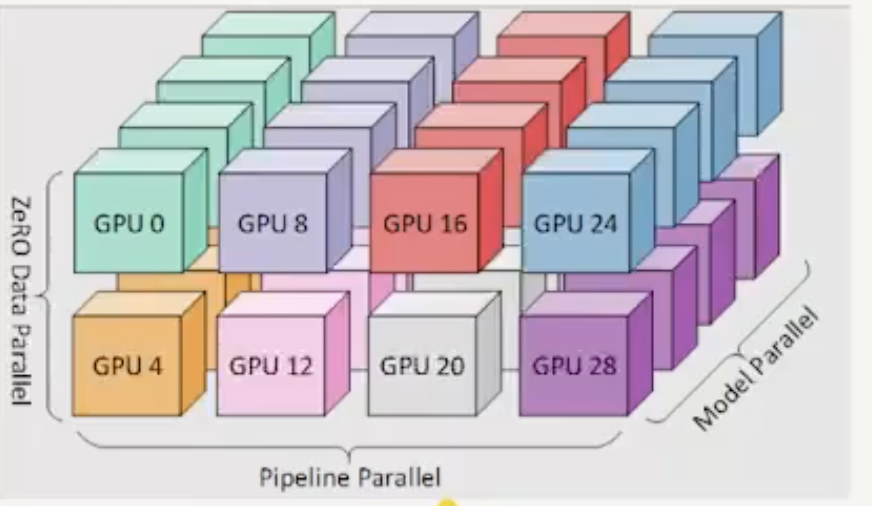
\includegraphics[width=0.95\linewidth]{zero.png}
\end{center}

\begin{center}
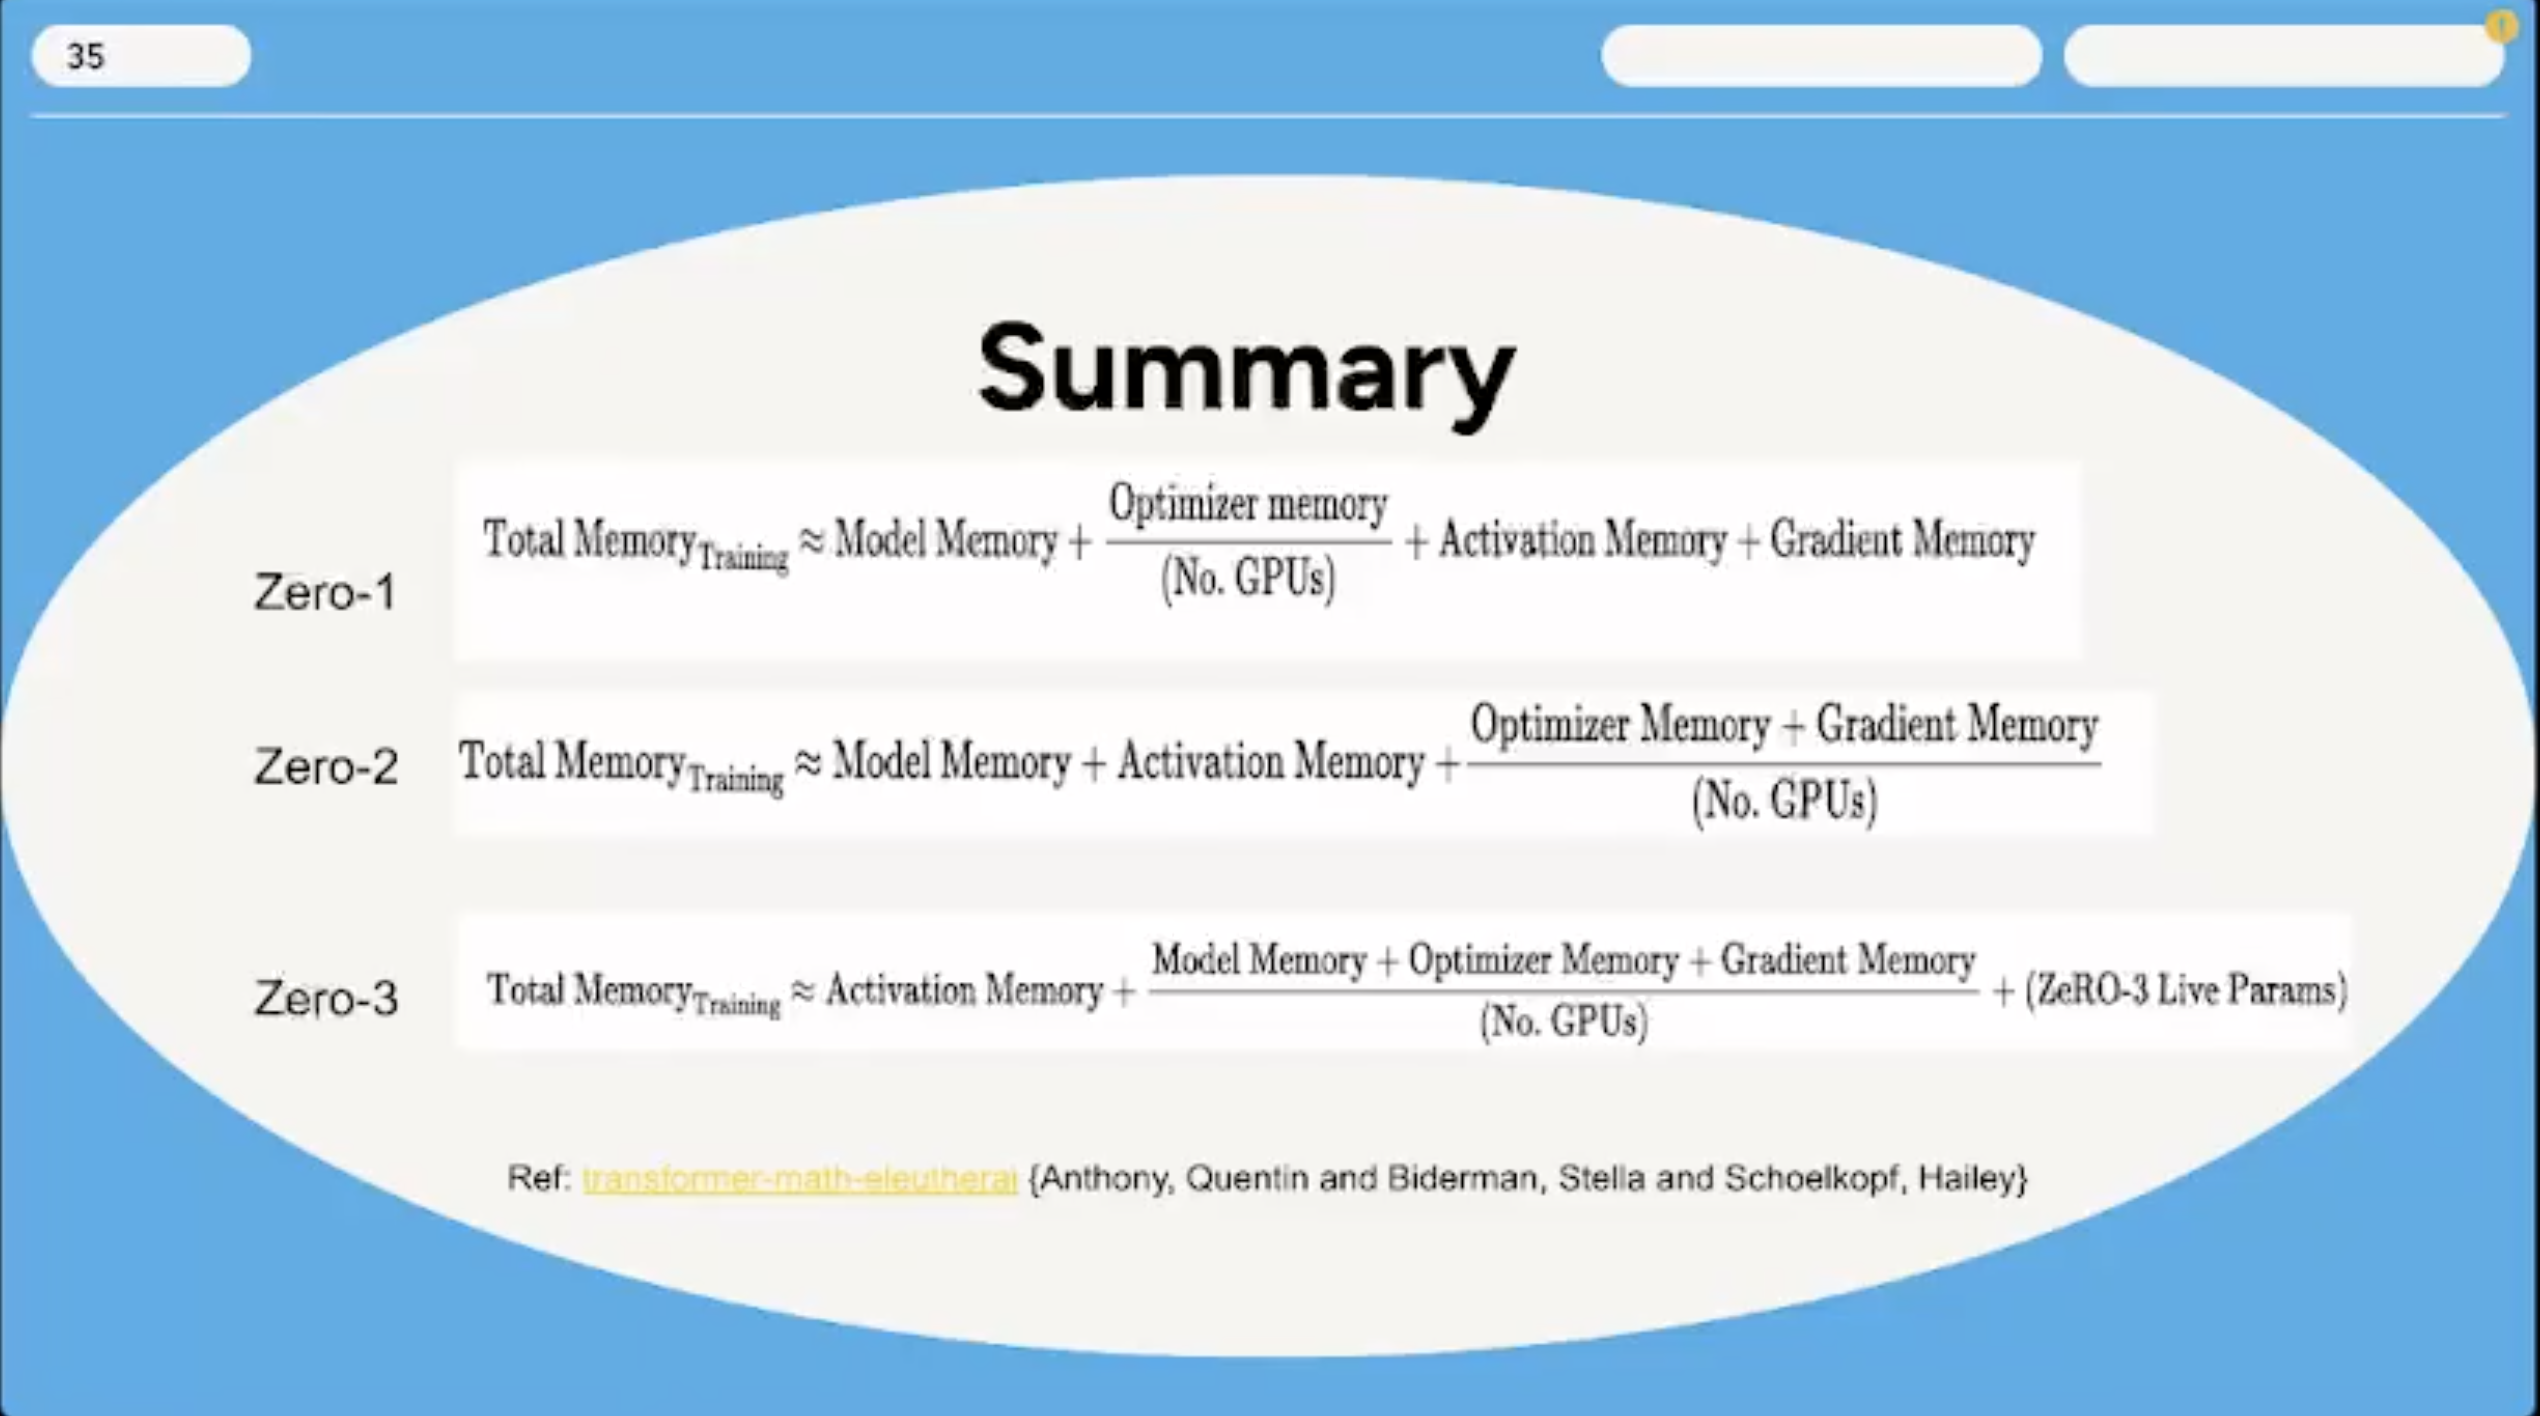
\includegraphics[width=0.95\linewidth]{sum.png}
\end{center}



\section{ \textbf{Session 4: Ring Attention}}

\begin{redbox}
\textbf{Session framing (preserved + cleaned):}
Ring self-attention v1 did not show a huge impact in all settings, but later versions (combined with blockwise parallel ideas) showed stronger memory and communication benefits.
\end{redbox}

\subsection{Scope (three papers/topics you listed)}
\begin{enumerate}[leftmargin=1.3em]
\item \textbf{Sequence Parallelism (Ring Self-Attention)}
\item \textbf{Blockwise Parallel Transformers}
\item \textbf{Third paper/topic (placeholder in your notes)}
\end{enumerate}

\subsection{Why this line of work exists}
\begin{itemize}[leftmargin=1.2em]
\item Long-context attention creates a major memory bottleneck.
\item Even with tensor/pipeline parallelism, very large sequence lengths remain expensive.
\item Goal: increase maximum context length while keeping communication and memory manageable.
\end{itemize}

\subsection{Sequence Parallelism via Ring Self-Attention (preserved + clarified)}
\begin{bluebox}
\textbf{Core mechanism:}
Partition the \blue{sequence dimension} across devices. Keep each device's local query block fixed, and rotate key/value blocks in a ring so each device can compute full attention output for its local queries.
\end{bluebox}

\textbf{Execution sketch (your idea, organized):}
\begin{enumerate}[leftmargin=1.3em]
\item Partition tokens across devices.
\item Compute local Q/K/V projections for each token shard.
\item For each device, keep local query block fixed.
\item Rotate key blocks around the ring:
  \begin{itemize}
  \item At each step, compute partial attention scores for current key block.
  \item Overlap compute with send/receive of next key block.
  \end{itemize}
\item After \(N-1\) ring steps (for \(N\) devices), each device has seen all key blocks for its local queries.
\item Rotate value blocks similarly and accumulate final attention outputs.
\end{enumerate}

\begin{importantbox}
\textbf{Misconception cleared:}
This is \red{not} linear-attention approximation. Ring attention still computes \textbf{exact attention} for each query; it changes \textbf{partitioning and communication pattern} to reduce per-device memory pressure and improve scalability.
\end{importantbox}

\subsection{Complexity and scaling intuition (cleaned from your notes)}
\begin{itemize}[leftmargin=1.2em]
\item Global attention remains quadratic in sequence length overall.
\item Per-device memory/working set is reduced via sequence partitioning.
\item Communication is structured ring exchange instead of full all-gather of all keys/values at once.
\item This can enable much longer contexts in practice (your note: up to \(\sim 114\)k tokens in reported setups).
\end{itemize}

\begin{center}
\renewcommand{\arraystretch}{1.15}
\begin{tabular}{|p{0.28\linewidth}|p{0.30\linewidth}|p{0.34\linewidth}|}
\hline
\textbf{Approach} & \textbf{What is partitioned} & \textbf{Main implication} \\
\hline
Tensor parallelism (baseline in your note) & Model weight tensors/matmul dimensions & Requires synchronization/all-gather patterns around sharded matmuls \\
\hline
Sequence parallelism (ring attention) & Token/sequence dimension & Keeps local query block fixed, rotates K/V blocks, lowers per-device sequence memory load \\
\hline
\end{tabular}
\end{center}

\subsection{Batch-size observation from your notes}
\begin{itemize}[leftmargin=1.2em]
\item You noted better efficiency when batch size is larger.
\item In your notes: multi-head attention with sequence parallelism looked more efficient for batch size \(>16\) in the studied setting.
\end{itemize}

\subsection{Blockwise Parallel Transformers (placeholder preserved)}
\begin{itemize}[leftmargin=1.2em]
\item Your note: this was a key reason later versions had stronger impact.
\item Working interpretation: blockwise execution helps sustain lower memory footprint and communication overhead.
\item Keep this section as a placeholder until paper-specific equations/algorithms are added.
\end{itemize}

\subsection{Third paper/topic (placeholder preserved)}
\begin{itemize}[leftmargin=1.2em]
\item Placeholder retained from original notes.
\item Add title + key contribution once finalized.
\end{itemize}

\section{\textbf{Session 8: Megatron-LM -- Training Multi-Billion-Parameter Models with Model Parallelism}}

\begin{bluebox}
\textbf{Session 8 thesis (your notes, organized):}\\
Megatron-LM combines \blue{tensor model parallelism} (intra-layer splits) with pipeline/data-parallel ideas to scale large Transformers while controlling communication overhead.
\end{bluebox}

\subsection{Why this paper mattered}
\begin{itemize}[leftmargin=1.2em]
\item The paper demonstrated strong scaling from smaller to much larger GPU counts.
\item Your notes emphasize this practical result: good scaling efficiency is achievable, but communication overhead is the main bottleneck to manage.
\item Goal: keep mathematically equivalent training while changing \textbf{where} and \textbf{when} communication occurs.
\end{itemize}

\begin{redbox}
\textbf{Guiding rule (preserved + clarified):}\\
Do not change model math; only change operation partitioning and synchronization timing.
\end{redbox}

\subsection{Transformer block decomposition used in the notes}
\begin{itemize}[leftmargin=1.2em]
\item Self-attention block
\item MLP block (two GEMMs with GELU nonlinearity in between)
\item Residual + dropout around sublayers
\end{itemize}

\subsection{Key MLP insight: avoid synchronization before GELU}
Your notes highlight a central design choice:
\begin{itemize}[leftmargin=1.2em]
\item If a split produces \textbf{partial sums} before a nonlinearity, applying GELU locally is not equivalent to applying GELU after global sum.
\item Therefore, that split forces an early all-reduce, which hurts performance.
\item Megatron chooses partitions that delay synchronization until after nonlinearity-safe points.
\end{itemize}

\begin{importantbox}
\textbf{Why early sync is bad here:}\\
For nonlinear \(f\), in general \(f(a+b)\neq f(a)+f(b)\).  
So if each GPU only has partial pre-activation sums, you must communicate before GELU to preserve exact math.
\end{importantbox}

\subsubsection*{\blue{MLP partition pattern (as reflected in your notes)}}
\begin{enumerate}[leftmargin=1.3em]
\item First projection GEMM: \textbf{column-parallel} split (each rank computes complete local outputs for its shard).
\item Apply GELU \textbf{locally} on each shard (safe, no immediate sync).
\item Second projection GEMM: \textbf{row-parallel} split.
\item All-reduce partial outputs at the end of the MLP block.
\end{enumerate}

\begin{bluebox}
\textbf{Recall line:} first GEMM column split, second GEMM row split, then synchronize once at block output.
\end{bluebox}

\subsection{Self-attention tensor parallelism (from your notes)}
\begin{itemize}[leftmargin=1.2em]
\item Exploit natural independence across attention heads.
\item Replicate input activation \(X\) across tensor-parallel ranks.
\item Shard Q/K/V projections by heads so each rank computes attention for its local head subset.
\item Perform local attention (\(QK^T\), softmax, \(PV\)) without intermediate cross-rank communication.
\item Project back to hidden dimension and all-reduce at the output projection stage.
\end{itemize}

\subsection{Communication pattern summary}
\begin{center}
\renewcommand{\arraystretch}{1.15}
\begin{tabular}{|p{0.32\linewidth}|p{0.28\linewidth}|p{0.30\linewidth}|}
\hline
\textbf{Block} & \textbf{Local compute} & \textbf{Synchronization point} \\
\hline
MLP & GEMM$_1$ + GELU + GEMM$_2$ (sharded) & All-reduce at block output \\
\hline
Self-attention & QKV + attention per local heads & All-reduce at output projection \\
\hline
\end{tabular}
\end{center}

Your note that this design uses a small number of all-reduces per Transformer layer (forward/backward) matches the core optimization target: fewer, well-placed synchronizations.

\subsection{Input and output embedding parallelism}
You captured an important memory point: the vocabulary embedding matrix is huge, so sharding by vocabulary dimension is beneficial.

\subsubsection*{\blue{Input embedding logic (filled + clarified)}}
\begin{itemize}[leftmargin=1.2em]
\item Split embedding table across vocabulary rows (each GPU owns a token-ID range).
\item For each token ID:
  \begin{itemize}
  \item If ID is in local shard range, perform local lookup.
  \item Otherwise, contribute zeros (masked lookup).
  \end{itemize}
\item Sum partial embedding contributions across ranks (all-reduce or reduce-scatter/all-gather variants depending on the parallel stack).
\item Result: every rank gets the correct full embedding activations while storing only a shard of the embedding table.
\end{itemize}

\subsubsection*{\blue{Output embedding / vocab logits logic (placeholder filled)}}
\begin{itemize}[leftmargin=1.2em]
\item Output projection is also vocabulary-sharded: each rank computes logits for its local vocab slice only.
\item Naively, full softmax would require gathering all vocab logits.
\item Megatron-style implementations avoid a full logits all-gather by fusing parallel logits with cross-entropy:
  \begin{itemize}
  \item compute local max/log-sum-exp contributions,
  \item reduce across ranks for global normalization terms,
  \item compute loss/gradients directly from sharded logits.
  \end{itemize}
\item This significantly reduces communication and memory traffic compared with materializing full vocab logits on every rank.
\end{itemize}

\begin{redbox}
\textbf{Misconception corrected:}
You usually do \textbf{not} need to all-gather the full vocabulary logits for cross-entropy in tensor-parallel training.  
Fused sharded cross-entropy computes the exact loss with reduced communication.
\end{redbox}

\subsection{Practical takeaway (your notes distilled)}
\begin{itemize}[leftmargin=1.2em]
\item Tensor model parallelism is most effective when communication stays mostly intra-node (high-bandwidth links).
\item Main design challenge is not splitting compute, but placing synchronization so nonlinear correctness is preserved and communication is minimized.
\item Vocabulary sharding and fused loss are crucial for scaling large-vocab LMs.
\end{itemize}
\section{\textbf{Session 16: LMCache}}

\begin{bluebox}
\textbf{Session 16 thesis (from your notes, cleaned):}\\
LMCache treats \blue{KV cache as a first-class system component} and combines it with
\blue{prefill/decode disaggregation} and \blue{paged attention} to improve end-to-end inference efficiency.
\end{bluebox}

\subsection{Motivation}
\begin{itemize}[leftmargin=1.2em]
\item Processing each user request fully independently is inefficient, especially with system prompts, multi-turn context, and long traces.
\item End-to-end serving has mixed phases: some are compute-bound (prefill), others are memory or communication-bound (decode).
\item Core goal: reuse prior compute (KV cache), minimize redundant work, and improve GPU utilization plus first-token latency.
\end{itemize}

\subsection{Why KV cache helps}
\textbf{Your original intuition, organized:} modern LLMs are decoder-based and generate tokens autoregressively.  
You feed in a prompt, the model runs it through many Transformer layers, and then predicts the next token.  
That next token is appended to the sequence, and the process repeats.

\begin{itemize}[leftmargin=1.2em]
\item Each layer produces \textbf{query}, \textbf{key}, and \textbf{value} vectors.
\item Attention uses queries against keys to produce scores, and then uses those scores to weight the values.
\item For the newest token, the only query we need is the query for that newest token, but it must attend over \textbf{all previous keys and values}.
\item Without caching, the system would keep recomputing old keys and values again and again at every decode step.
\end{itemize}

\begin{addedbox}
\textbf{Correction added:}\\
KV cache stores \textbf{keys and values}, not queries. Query vectors are computed for the current token at decode time.
\end{addedbox}

\textbf{Redundant-work picture (preserved + clarified):}
\begin{itemize}[leftmargin=1.2em]
\item Generating token 50 requires access to K/V for tokens \(1 \dots 50\).
\item Generating token 51 requires access to K/V for tokens \(1 \dots 51\).
\item If you recompute all prior K/V every step, you are repeating a huge amount of projection work.
\end{itemize}

\textbf{So the fix is:}
\begin{enumerate}[leftmargin=1.3em]
\item Compute Q/K/V for only the newest token.
\item Append the new K and V to the cache.
\item Retrieve the previously cached K/V for all earlier tokens.
\item Run attention using the new query against the full cached history.
\end{enumerate}

\begin{redbox}
\textbf{Important compute intuition:}\\
KV caching removes repeated \textbf{projection work} for past tokens, but decode still scales with sequence length because each new token still attends over all cached history.
\end{redbox}

\subsection{Prefill, decode, and TTFT}
\textbf{Your original reasoning chain:}
\begin{itemize}[leftmargin=1.2em]
\item The first token is slow because the model must process the entire prompt first.
\item That first full pass computes and stores K/V for every prompt token.
\item This is the \blue{prefill phase}, and it is the most compute-intensive part of the request.
\item Once the cache is warm, later tokens only need a one-token decode step, so generation becomes much cheaper.
\end{itemize}

\begin{center}
\renewcommand{\arraystretch}{1.15}
\begin{tabular}{|p{0.23\linewidth}|p{0.33\linewidth}|p{0.34\linewidth}|}
\hline
\textbf{Phase} & \textbf{What happens} & \textbf{Why it matters} \\
\hline
Prefill & Full prompt forward pass, build KV cache & Dominates first-token latency \\
\hline
Decode & One-token step using cached history & Cheaper per token, but memory-sensitive \\
\hline
\end{tabular}
\end{center}

\textbf{TTFT (time to first token):}
\begin{itemize}[leftmargin=1.2em]
\item Longer prompt $\Rightarrow$ longer prefill.
\item Longer prefill $\Rightarrow$ longer wait before the first generated token.
\item This is why TTFT optimization is its own topic: chunked prefill, speculative decoding, and prompt caching all target this initial delay.
\end{itemize}

\begin{bluebox}
\textbf{Recall line:}\\
Building the cache is expensive. Reading from the cache is cheap.
\end{bluebox}

\subsection{Memory tradeoff of KV cache}
\begin{itemize}[leftmargin=1.2em]
\item KV caching trades \blue{compute savings} for \red{memory usage}.
\item Every layer stores K/V tensors for every token in the active context.
\item As context length increases, KV cache grows linearly with sequence length.
\item At high concurrency, KV memory can become one of the dominant serving costs.
\end{itemize}

\textbf{Your original concern, preserved:}
\begin{itemize}[leftmargin=1.2em]
\item For long-context models and many concurrent requests, KV cache can become so large that it rivals or exceeds model-weight memory.
\item This is one reason \blue{MQA} and \blue{GQA} exist: they reduce the number of key/value heads that must be stored.
\item Doubling context length is hard in practice partly because it also doubles per-request KV-cache footprint.
\end{itemize}

\subsection{Prefill/decode disaggregation (PD disaggregation)}
\textbf{Your original system-level point:} prefill and decode are very different workloads, so it often makes sense to split them.

\begin{itemize}[leftmargin=1.2em]
\item Prefill is dense-matrix heavy and benefits from high-throughput accelerators.
\item Decode is token-by-token, latency-sensitive, and often bottlenecked by memory movement plus cache access.
\item Splitting these phases across different workers/devices can improve throughput and cost-efficiency, depending on workload.
\item The decode-side requirement is enough fast memory capacity/bandwidth to serve KV cache efficiently.
\end{itemize}

\begin{addedbox}
\textbf{Added nuance:}\\
PD disaggregation is powerful for large or mixed workloads, but can be overkill for smaller models or low concurrency where transfer overhead dominates.
\end{addedbox}

\textbf{How you were thinking about it (preserved + cleaned):}
\begin{itemize}[leftmargin=1.2em]
\item You do not want to waste the same GPU doing both heavy prompt processing and low-throughput token streaming if those phases want different hardware characteristics.
\item Prefill can run on a large, throughput-oriented GPU.
\item Decode may be cheaper to run on a device optimized for fast cache access and serving latency.
\item LMCache makes this practical by letting prefill produce cache and decode consume it elsewhere.
\end{itemize}

\subsection{Paged attention and cache paging}
\textbf{Your original motivation:} systems do not want to move or allocate memory one token at a time if the transport and allocator both prefer chunked operations.

\begin{itemize}[leftmargin=1.2em]
\item Variable-length requests can cause memory fragmentation if KV memory is managed as large contiguous buffers.
\item Paged attention uses fixed-size pages from a shared pool and maps each request to a list of pages.
\item This improves reuse and flexibility: pages for shared prefixes (for example, common system prompts) can be reused.
\item Data movement is performed in page-sized chunks instead of tiny per-token transfers.
\end{itemize}

\textbf{Your original allocator intuition, organized:}
\begin{itemize}[leftmargin=1.2em]
\item If every request gets a custom-sized contiguous buffer, memory becomes fragmented.
\item Fixed-size pages are easier to reuse, move, and share.
\item A request effectively becomes a list of pages rather than one giant flat tensor buffer.
\item Shared system prompts are especially attractive because those pages may be reusable across many requests.
\end{itemize}

\subsection{LMCache design philosophy (from your notes)}
\begin{itemize}[leftmargin=1.2em]
\item Treat KV cache as a first-class object (move, pin, evict, compress, and tier it explicitly).
\item I/O-aware operation: batch and size transfers near each device/link sweet spot.
\item Modular interface: a common API that multiple inference engines can call.
\item Explicit cache control enables better coordination with prefill/decode split pipelines.
\end{itemize}

\subsection{System architecture}
\begin{itemize}[leftmargin=1.2em]
\item \textbf{Cache controller:} API-facing control plane (router/scheduler interaction).
\item \textbf{Worker process:} data plane that moves/manages cache across GPU memory and storage backends.
\item This architecture supports distributed deployment across multiple hosts/instances.
\end{itemize}

\subsection{Request lifecycle (organized from your steps)}
\textbf{Your original request flow, restored in order:}
\begin{enumerate}[leftmargin=1.3em]
\item \textbf{Request arrival + metadata routing:} identify reusable cache and choose target worker/device.
\item \textbf{Page allocation plan:} reuse existing pages, allocate missing pages, prepare transfer plan.
\item \textbf{KV load + prefill overlap:} pipeline cache transfer and compute so later-layer cache can arrive while earlier layers run.
\item \textbf{Decode/token generation:} generate tokens incrementally while updating/transferring KV in batches.
\item \textbf{Response + cleanup:} return tokens, update cache metadata, evict or persist pages by policy.
\end{enumerate}

\textbf{Step-by-step interpretation from your notes:}
\begin{itemize}[leftmargin=1.2em]
\item When a request arrives, the scheduler/router asks whether relevant cache already exists somewhere in the system.
\item If cache exists, the system decides which worker/device is best positioned to use it.
\item It allocates or reuses pages, then starts pulling the needed cache toward the compute path.
\item Cache loading can overlap with prefill/compute so the next layer's data is arriving while the current layer is executing.
\item During generation, KV updates are batched and transferred in page groups rather than tiny fragmented writes.
\item After the request finishes, the system decides what to keep hot, what to evict, and what to push to colder tiers.
\end{itemize}

\subsection{Recompute vs fetch decision}
\begin{itemize}[leftmargin=1.2em]
\item A practical scheduler decision is whether to recompute context or fetch existing KV from another tier/device.
\item The crossover point depends on interconnect and topology (NVLink, PCIe, TCP/RDMA, single-node vs multi-node) and target first-token latency.
\item LMCache-style systems use cost models to avoid moving very small chunks inefficiently.
\end{itemize}

\textbf{Your original performance question, preserved:}
\begin{itemize}[leftmargin=1.2em]
\item Sometimes it is cheaper to recompute than to fetch.
\item Sometimes it is cheaper to fetch existing KV than to rebuild it.
\item The answer depends on topology and transfer path: NVLink, PCIe, TCP, multi-node, single-node, and the amount of data.
\item This is especially important if the system is optimizing for first-token latency.
\end{itemize}

\subsection{Tiered storage and key optimizations}
\begin{itemize}[leftmargin=1.2em]
\item Tiered cache (GPU memory, CPU memory, and colder storage tiers) based on hot/cold access patterns.
\item Batched data movement in chunks/pages to improve effective bandwidth.
\item Layer-wise pipelining: overlap KV loading with compute.
\item Zero-copy style transfers where possible to reduce duplication.
\item Asynchronous prefetch for queued requests during idle windows.
\end{itemize}

\textbf{Your original key optimizations, rewritten but preserved:}
\begin{itemize}[leftmargin=1.2em]
\item \textbf{Batched data movement:} move chunks/pages instead of many tiny pieces.
\item \textbf{Layer-wise pipelining:} load cache for the next layer while the current layer computes.
\item \textbf{Zero-copy direction:} minimize duplicate copies during transfer.
\item \textbf{Async prefetch:} load likely-needed cache during idle time.
\item \textbf{Storage hierarchy management:} keep hot context close (GPU/CPU memory), push cold context farther away.
\end{itemize}

\subsection{Quick recall table}
\begin{center}
\renewcommand{\arraystretch}{1.15}
\begin{tabular}{|p{0.30\linewidth}|p{0.30\linewidth}|p{0.30\linewidth}|}
\hline
\textbf{Concept} & \textbf{Main benefit} & \textbf{Main tradeoff} \\
\hline
KV caching & Avoids redundant prefill compute & Consumes memory capacity \\
\hline
PD disaggregation & Better device specialization/utilization & Extra coordination + transfer overhead \\
\hline
Paged attention & Less fragmentation, better reuse & Added page-management complexity \\
\hline
Tiered cache & Larger effective cache capacity & Eviction/prefetch policy tuning needed \\
\hline
\end{tabular}
\end{center}

\begin{redbox}
\textbf{Performance takeaway (from your notes, cleaned):}\\
LMCache-style systems can outperform naive black-box caching pipelines because they are explicitly optimized for
I/O patterns, cache placement, and overlap of transfer with compute, even when implemented in Python control layers.
\end{redbox}
\subsection{Video 5: Paged Attention and vLLM-style Serving}

\begin{bluebox}
\textbf{Why this matters for inference:}\\
In serving, the real bottleneck is often not just model weights. It is the \blue{dynamic KV-cache state} that grows with requests and limits throughput.
\end{bluebox}

\textbf{Your original split between phases, organized:}
\begin{itemize}[leftmargin=1.2em]
\item \textbf{Prefill:} generate KV vectors for the full prompt.
\item \textbf{Decode:} generate new tokens one at a time using existing KV cache.
\item Prefill is compute-heavy and parallel-friendly.
\item Decode is much more memory-bound because it must keep and read growing KV state.
\end{itemize}

\textbf{System-level implication from your notes:}
\begin{itemize}[leftmargin=1.2em]
\item Model weights are mostly static memory.
\item KV cache is dynamic memory that grows and shrinks with active requests.
\item As request count and context length increase, KV cache can become the main factor limiting batch size and throughput.
\end{itemize}

\subsection{Why contiguous KV-cache allocation breaks down}
\textbf{Your original concern, cleaned:} many serving systems historically allocated one contiguous chunk of memory per request for KV cache.

\begin{itemize}[leftmargin=1.2em]
\item If a system reserves space for future output tokens up front, much of that space may sit unused for a while.
\item If requests have different prompt lengths and different generation lengths, the allocator ends up with uneven free gaps.
\item This leads to both \blue{internal fragmentation} and \blue{external fragmentation}.
\end{itemize}

\begin{center}
\renewcommand{\arraystretch}{1.15}
\begin{tabular}{|p{0.23\linewidth}|p{0.31\linewidth}|p{0.34\linewidth}|}
\hline
\textbf{Type} & \textbf{What it means} & \textbf{In KV-cache serving} \\
\hline
Internal fragmentation & Reserved block is bigger than actually used data & Request gets extra KV space that sits idle until later tokens arrive \\
\hline
External fragmentation & Free memory exists but is split into awkward gaps & System has total free memory, but not in the right shapes for new requests \\
\hline
\end{tabular}
\end{center}

\begin{addedbox}
\textbf{OS analogy made explicit:}\\
Paged attention is inspired by virtual memory.  
Requests behave like processes, KV blocks behave like pages, and the system maps a request's \textbf{logical} KV layout to \textbf{physical} memory blocks that do not need to be contiguous.
\end{addedbox}

\subsection{Paged attention idea}
\begin{itemize}[leftmargin=1.2em]
\item Instead of one giant contiguous region per request, KV cache is split into fixed-size blocks.
\item Logical token order remains contiguous from the model's perspective.
\item Physical storage can live in non-contiguous blocks in memory.
\item This allows the allocator to fill memory incrementally as requests grow token by token.
\end{itemize}

\textbf{What this improves from your notes:}
\begin{itemize}[leftmargin=1.2em]
\item Less external fragmentation because the system can place blocks wherever space exists.
\item Less waste from over-reserving huge contiguous regions.
\item Better sharing opportunities between related outputs, such as beam search, parallel sampling, or prefix reuse.
\end{itemize}

\begin{redbox}
\textbf{Important clarification:}\\
Paged attention is mainly a \textbf{memory-management and serving-systems optimization}.  
It does not change the Transformer math the way FlashAttention changes how attention is computed on-chip.
\end{redbox}

\subsection{Continuous batching and decode scheduling}
\textbf{Your notes were getting at two batching ideas:}
\begin{itemize}[leftmargin=1.2em]
\item \textbf{Continuous batching:} scheduling decisions are made at each decode iteration, so finished requests leave and new requests can join without waiting for an entire static batch to finish.
\item \textbf{Mixed batching:} some requests may be in prefill while others are already in decode.
\end{itemize}

\textbf{Why this matters:}
\begin{itemize}[leftmargin=1.2em]
\item Decode runs token by token, so a static batch wastes capacity whenever some requests finish early.
\item Continuous batching keeps the GPU busier by filling those open slots quickly.
\item Paged attention makes this practical because memory is managed in smaller blocks rather than rigid per-request slabs.
\end{itemize}

\subsection{vLLM-style implementation picture}
\textbf{Your original architecture ideas, organized:}
\begin{itemize}[leftmargin=1.2em]
\item A \blue{central scheduler} coordinates which requests run and when.
\item A \blue{KV-cache manager} tracks logical-to-physical block mappings.
\item The cache manager knows which blocks are free, allocates new ones, and appends blocks as a request grows.
\item Scheduler policy depends on block size, free memory, model length, and whether prefix caching or sliding-window behavior is enabled.
\end{itemize}

\textbf{Why this kicked off vLLM in practice:}
\begin{itemize}[leftmargin=1.2em]
\item It made much better use of HBM during decode.
\item It reduced memory waste enough to support larger effective batches and higher serving throughput.
\item It exposed the fact that decode throughput is often constrained more by KV-cache management than by raw FLOPs.
\end{itemize}

\subsection{Sharing and branching outputs}
\begin{itemize}[leftmargin=1.2em]
\item Beam search and parallel sampling create multiple outputs that share a prefix.
\item In naive serving, each output may duplicate the same prefix KV cache.
\item With block-level management, those shared prefix blocks can be reused instead of copied immediately.
\item This is one of the reasons paged/block-based cache management helps much more than just ``packing memory better.''
\end{itemize}

\subsection{Single-instance vs multi-instance serving}
\textbf{Your original notes moved from one-device systems to fleets. That distinction matters:}
\begin{itemize}[leftmargin=1.2em]
\item Inside a single serving instance, the scheduler and cache manager directly control GPU memory.
\item In a fleet, you need a higher-level orchestrator to decide where requests go and how cache locality is preserved.
\item This is where disaggregated serving, routing, and cache transfer become important.
\end{itemize}

\textbf{Examples from your notes:}
\begin{itemize}[leftmargin=1.2em]
\item A prefill server can compute KV cache and send it to a decode server.
\item Orchestration above the model server may be done with systems like Kubernetes or Slurm.
\item Once you have many instances, ordinary round-robin load balancing is not enough if cache locality matters.
\end{itemize}

\begin{addedbox}
\textbf{Session affinity filled in:}\\
\blue{Session affinity} means routing follow-up requests from the same session/user to the same backend instance whenever possible, so cached state (especially KV cache or conversation context) can be reused locally instead of transferred or recomputed.
\end{addedbox}

\subsection{Multi-host serving notes}
\begin{itemize}[leftmargin=1.2em]
\item A single large model can itself use model parallelism across hosts.
\item On top of that, you may also run multiple replicated serving instances behind a load balancer.
\item Some features, like speculative decoding, may involve multiple models with different hardware needs.
\item In those cases, you care a lot about which path is latency-critical and which path can tolerate extra network hops.
\end{itemize}

\textbf{Your original systems intuition, preserved:}
\begin{itemize}[leftmargin=1.2em]
\item Keep the fast path extremely fast.
\item Let the slow or fallback path absorb more latency if necessary.
\item Different models may need different hardware and different scaling strategies.
\end{itemize}

\subsection{Final paged-attention memory intuition}
\begin{itemize}[leftmargin=1.2em]
\item Logical KV order for a request stays clean and contiguous from the model's perspective.
\item Physical memory allocation is block-based and can be non-contiguous.
\item The last partially filled block can be extended by future tokens of the same request.
\item Requests with shared prefixes may share earlier blocks before diverging.
\end{itemize}

\begin{bluebox}
\textbf{Exam recall line:}\\
FlashAttention is about \blue{compute-efficient attention on GPU}.  
Paged attention is about \blue{memory-efficient KV-cache management for serving}.
\end{bluebox}






\bigspace
\end{document}
